\chapter{Appendix}

To run the code, there has to be installed only Python 3 (with various libraries) on any OS. All the Python code can be found in the directory \texttt{src/}. The entire project is open-source and can be found as a public \href{https://github.com/KuboBahyl/superfluid}{GitHub} repository. Pull requests of any further development would be definitely appreciated.

Here we briefly present a few visualisations of observed instabilities and physical processes.

\subsection*{Instability in good resolution}


\begin{figure}[h]
	\centering
	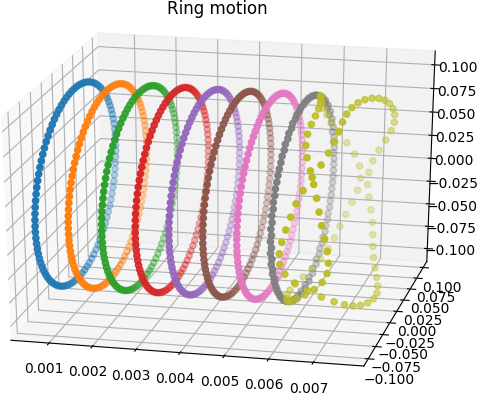
\includegraphics[width=0.6\textwidth]{graphics/results/euler_instability}
	\caption{A graphical example of ring instability when Euler stepping was used with good resolution (small $\delta$). Ring is moving from the left side to the right with exponentially forwarding error.}
\end{figure}

\subsection*{Noisy instability in worse resolution}

\begin{figure}[h]
	\centering
	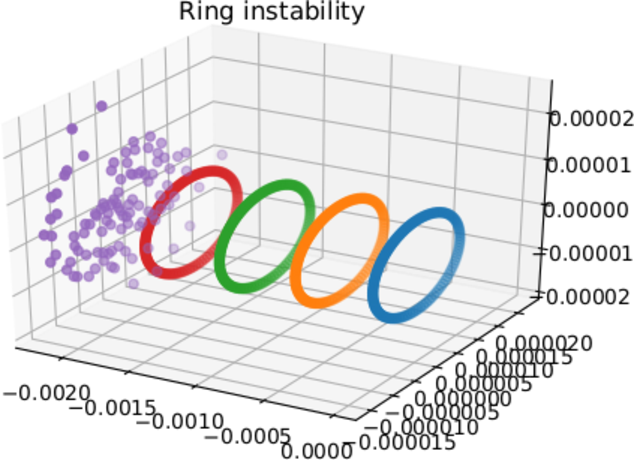
\includegraphics[width=0.6\textwidth]{graphics/results/ring-instability}
	\caption{Another example of ring instability due to forwarded numerical error using Euler stepping. In this case, resolution $\delta$ is higher (worse resolution), so the instability itself is much more noisy.}
\end{figure}

\newpage

\subsection*{Mutual frtiction effects}

Also, we present one of the bigger simulations (\textbf{Figure 17}) we tested. After we set the ring radius $R=1000\mu\text{m}$, resolution $\delta=60\mu\text{m}$ (resulting in around $\approx$ 100 mesh points),
re-segmentation boundaries $\delta_{\text{min}}= \delta /2 = 30\mu\text{m}$, $\delta_{\text{max}} = 2\delta = 120\mu\text{m}$, the updated LIA calculation, RK4 stepping method and a temperature $T=1.5\text{K}$, we obtained a stable simulation of vortex ring with a decreasing radius. More on particular physical processes can be found in \cite{biot_origin}.

\begin{figure}[h]
	\centering
	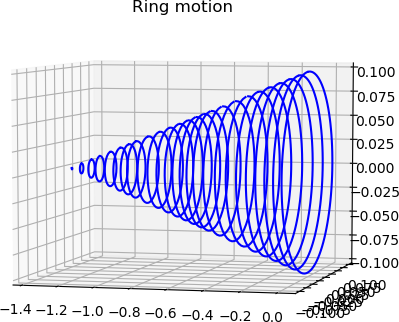
\includegraphics[width=0.6\textwidth]{graphics/results/ring-motion_full}
	\caption{Here, a vortex ring is moving to the left, its energy is dissipating due to the mutual friction and therefore, the radius is decreasing in time. The ring re-segmented itself a few times (due to the violation of $\delta_{\text{min}}$ condition and died (the simulation was stopped) when the length error was too high.}
\end{figure}

The last plot we show in \textbf{Figure (\ref{flow_phase})} is the \textit{flow phase diagram}, summarizing
all measured oscillators and their critical Donnelly numbers and critical dimensionless velocities. We also marked our estimated areas, where the transitions to non-linear regimes emerge.

\begin{figure}[h]
	\centering
	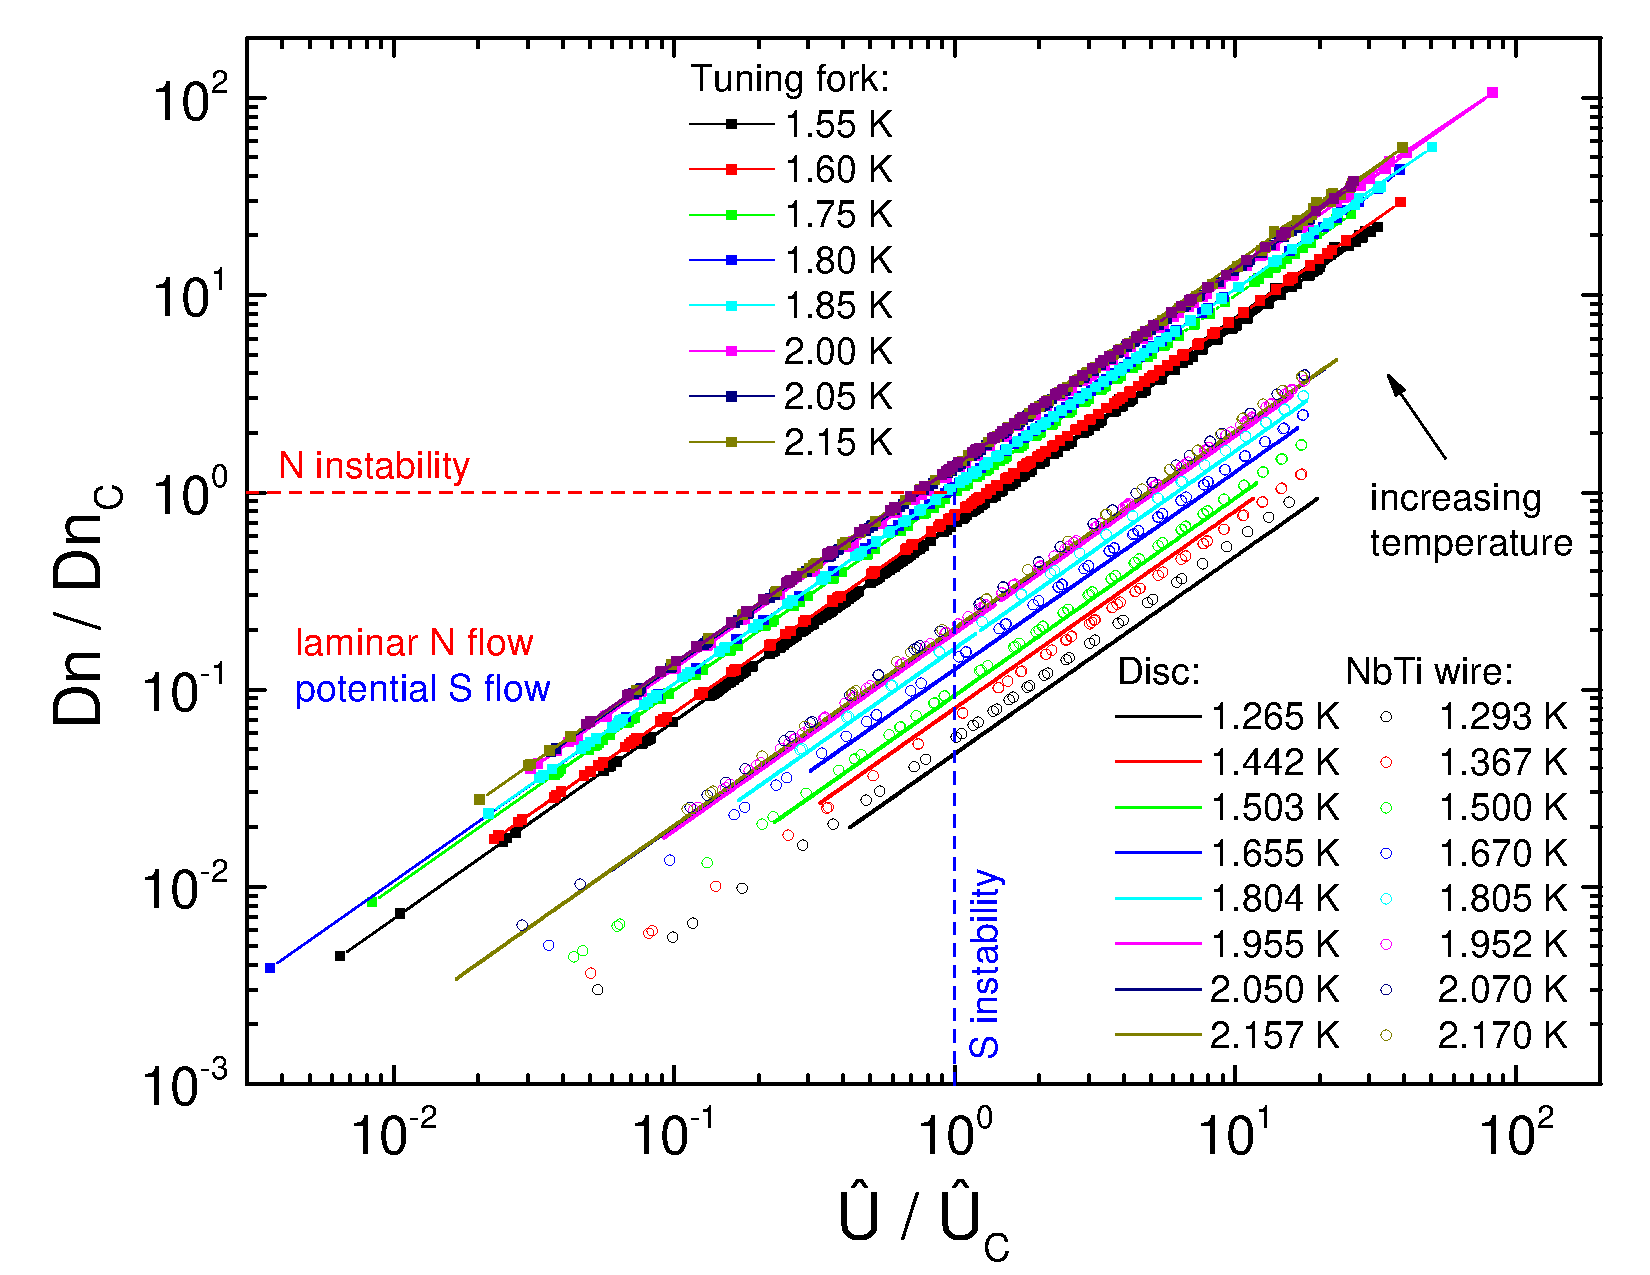
\includegraphics[width=0.8\textwidth]{graphics/results/flow_phase_diagram}
	\caption{Plot of scaled critical Donnelly numbers and critical dimensionless velocities for for all used oscillators. \underline{Dashed lines} marks the areas of transition from laminar/potential regimes to the non-linear ones, both for normal and superfluid components. }
	\label{flow_phase}
\end{figure}

\newpage
